% Split-Resurgence: The Splitter Analytics Gap
% Build:  tectonic paper/split_resurgence.tex   (from the repo root)
\documentclass[11pt]{article}

\usepackage[margin=1in]{geometry}
\usepackage[T1]{fontenc}
\usepackage{lmodern}
\usepackage{microtype}
\usepackage{amsmath}
\usepackage{booktabs}
\usepackage{graphicx}
\usepackage{caption}
\usepackage{xcolor}
\usepackage{enumitem}
\usepackage{xurl}
\usepackage[hidelinks]{hyperref}

\graphicspath{{../reports/figures/}{reports/figures/}}
\captionsetup{font=small,labelfont=bf}
\setlist{itemsep=2pt,topsep=4pt}

% --- Reported numbers (single source of truth for the text) ----------------
% npb_years, FS MixedLM
\newcommand{\npbEst}{0.101}
\newcommand{\npbAsymLo}{-0.096}
\newcommand{\npbAsymHi}{0.298}
\newcommand{\npbBootLo}{-0.114}
\newcommand{\npbBootHi}{0.250}
\newcommand{\npbBootN}{1,964}
\newcommand{\npbBootPos}{90\%}

\newcommand{\code}[1]{\texttt{#1}}
\newcommand{\FS}{\textsc{fs}}
\newcommand{\CH}{\textsc{ch}}

\title{\textbf{The Splitter Analytics Gap}\\[4pt]
\large Do Physics-Based Run-Value Models Miss Something About the Splitter,\\
and Does NPB Development Explain It?}
\author{Kylan Huynh}
\date{October 2026}

\begin{document}
\maketitle

\begin{abstract}
\noindent
Dodgers manager Dave Roberts said in 2025 that ``the analytics hasn't caught up to the split.'' We test one part of that claim with Statcast pitch-level data from 2021 through 2025 (3,614,368 pitches). An XGBoost model trained only on the physical characteristics of each pitch predicts per-pitch run value. Its out-of-fold residuals, aggregated to pitcher-seasons, define \emph{model resistance}: how much better a pitcher's pitch performed than physics alone predicts. A linear mixed model with a random pitcher intercept regresses splitter model resistance on years spent in Nippon Professional Baseball (NPB), MLB experience, fastball velocity, usage share, and a debut-season indicator, and we refit the same model on changeups for comparison. We find no detectable NPB-development effect: the estimate is $+\npbEst$ runs per 100 pitches per NPB year, with a pitcher-level cluster-bootstrap 95\% interval of $[\npbBootLo, \npbBootHi]$. Three other patterns stand out. Pitcher-specific variance in model resistance is about 2.4 times larger for splitters than for changeups. Debut-season pitchers underperform the model on splitters ($-0.87$, $p=0.03$) but not on changeups. Higher usage predicts outperformance on both pitches by similar amounts. None of the five NPB-trained pitchers in the sample throws enough changeups to be estimated on that pitch at all. Taken together, the splitter carries more pitcher-specific value than physics captures, but the data cannot attribute that value to NPB development.
\end{abstract}

% ===========================================================================
\section{Introduction}

\begin{quote}
\itshape ``I don't think the analytics has caught up to the split. It doesn't register as well with models. It's like a slow fastball. The split is so unique and it doesn't take into account a hitter's approach against it.''
\upshape\\\hfill--- Dave Roberts, to Jeff Passan, 2025~\cite{passan2025}
\end{quote}

The splitter has returned to Major League Baseball. In our data its share of regular-season pitches doubled from 1.61\% in 2021 to 3.26\% in 2025. In the 2025 postseason it reached 7.2\% of pitches, and batters hit .149/.208/.246 against it over roughly 290 plate appearances. Much of the growth comes from pitchers trained in Nippon Professional Baseball (NPB), where the pitch stayed standard while MLB organizations discouraged it over injury concerns.

Roberts' remark makes three separable claims: (i) run-value models undervalue the splitter; (ii) its physical signature resembles a fastball for longer than other off-speed pitches do; and (iii) models ignore the hitter's cognitive response. This paper tests (i) directly, addresses (ii) partially through tunneling figures and velocity-differential features, and leaves (iii) for future work.

A natural question is whether NPB-developed splitters beat the models more than domestic ones. That comparison is underpowered and confounded. Only five NPB-developed pitchers throw 100 or more splitters in any season of our window, only elite NPB pitchers are posted to MLB, and some domestic pitchers, Kevin Gausman most obviously, throw elite splitters. We therefore ask a broader question:

\begin{quote}
\emph{What physical and contextual features of a splitter predict its resistance to pitch-grading models, and does NPB development add explanatory power once those features are controlled for?}
\end{quote}

Treating NPB experience as one covariate among several lets the data weigh it against the alternatives.

% ===========================================================================
\section{Data}

\paragraph{Pitch data.} We use every regular-season and postseason pitch tracked by Statcast from 2021 through 2025, retrieved with \code{pybaseball}~\cite{pybaseball} in monthly chunks and cached locally. Each pitch carries Statcast's base-out-aware run value \code{delta\_run\_exp}, which is the dependent variable throughout.

\paragraph{Pitch types.} The analysis covers splitters (\FS) and changeups (\CH). The changeup is the natural comparison: if an effect appears on both pitches, it describes off-speed pitching in general rather than the splitter. Fastballs (four-seam, sinker, cutter) are included as training data for the baseline model.

\paragraph{Focal roster.} Ten pitchers are hand-curated (Table~\ref{tab:roster}). NPB years and MLB debut come from Baseball-Reference and NPB records. Debut years for all other pitchers come from the Chadwick Bureau register~\cite{chadwick}. Pitchers outside the focal roster are assigned zero NPB years.

\begin{table}[h]
\centering\small
\caption{Focal roster.}
\label{tab:roster}
\begin{tabular}{@{}llcc@{\qquad}llc@{}}
\toprule
\multicolumn{4}{c}{NPB-developed} & \multicolumn{3}{c}{Domestic} \\
\cmidrule(r){1-4}\cmidrule(l){5-7}
Pitcher & & NPB yrs & Debut & Pitcher & & Debut \\
\midrule
Yoshinobu Yamamoto & & 7 & 2024 & Kevin Gausman & & 2013 \\
Shohei Ohtani$^{a}$ & & 5 & 2018 & Nathan Eovaldi & & 2011 \\
Shota Imanaga & & 8 & 2024 & Paul Skenes & & 2024 \\
Roki Sasaki & & 4 & 2025 & Taijuan Walker & & 2012 \\
Kodai Senga & & 11 & 2023 & Trey Yesavage & & 2025 \\
\bottomrule
\multicolumn{7}{@{}l}{\footnotesize $^{a}$Pitching seasons through 2023 only.}
\end{tabular}
\end{table}

% ===========================================================================
\section{Methods}

\subsection{Physics-only baseline}

A single gradient-boosted regressor (XGBoost~\cite{xgboost}) predicts \code{delta\_run\_exp} for every \FS, \CH\ and fastball pitch. Its inputs are physical and situational only: release speed; horizontal and vertical movement; release position and extension; Statcast's initial-velocity and acceleration components; spin rate and axis; plate location; balls and strikes; batter and pitcher handedness; pitch type; and two engineered terms, each pitch's velocity and vertical-movement difference from the pitcher-season's primary fastball (the most frequent of four-seam, sinker or cutter). Pitcher and batter identities are excluded, so anything pitcher-specific that physics misses remains in the residual.

Predictions are out-of-fold from five-fold \code{GroupKFold} cross-validation grouped by (pitcher, season), so no pitcher-season is predicted by a model that saw it. Hyperparameters are deliberately modest (400 trees, depth 6, learning rate 0.05, row subsample 0.7). An aggressively tuned baseline would absorb part of the pitcher-level signal the regression needs. Out-of-fold RMSE is 0.224 runs, and the mean residual is approximately zero.

For each (pitcher, season, pitch type) cell with at least 100 pitches we define
\begin{equation}
\text{model resistance} = -100 \times \frac{1}{n}\sum_{i=1}^{n}\bigl(y_i - \hat y_i\bigr),
\end{equation}
where $y_i$ is \code{delta\_run\_exp}. Statcast's run value is signed so that lower is better for the pitcher, so positive model resistance means the pitcher's pitch did better than physics predicts. Units are runs per 100 pitches (RV/100).

\subsection{Mixed-effects regression}

For each pitch type $k \in \{\FS, \CH\}$, with pitcher $j$ in season $t$:
\begin{equation}
\begin{aligned}
\text{MR}_{jt} = {} & \beta_0 + \beta_1\,\text{npb\_years}_j + \beta_2\,\text{mlb\_seasons\_in}_{jt} + \beta_3\,\text{fb\_velo}_{jt} \\
& + \beta_4\,\text{usage\_share}_{jt} + \beta_5\,\text{debut\_season}_{jt} + u_j + \varepsilon_{jt},
\end{aligned}
\end{equation}
with $u_j \sim N(0, \sigma_u^2)$ and $\varepsilon_{jt} \sim N(0, \sigma^2)$. Here \code{mlb\_seasons\_in} is years since MLB debut, \code{fb\_velo} is mean primary-fastball velocity, \code{usage\_share} is the pitch's share of all pitches the pitcher threw that season, and \code{debut\_season} indicates the MLB debut year. Models are fit by REML in \code{statsmodels}~\cite{statsmodels}. The FS sample has 239 pitcher-seasons from 111 pitchers, eight of them from the five NPB-developed pitchers. The CH sample has 1,166 pitcher-seasons from 520 pitchers. Because many pitchers contribute a single season, the default L-BFGS optimizer meets a singular Hessian on the FS data, and the fit falls back to BFGS, which converges.

\subsection{Cluster bootstrap for the NPB coefficient}

The asymptotic standard error on $\beta_1$ treats eight rows as eight independent pieces of information, when they come from five pitchers. We therefore resample the 111 pitchers with replacement 2,000 times, relabeling duplicated pitchers as distinct groups, refit the model, and take the 2.5th and 97.5th percentiles of $\hat\beta_1$~\cite{cameron2008,field2007}. Resamples that contain no NPB pitcher leave $\beta_1$ unidentified and are discarded. All other coefficients rest on hundreds of pitcher-seasons, and we report their asymptotic intervals.

% ===========================================================================
\section{Results}

\subsection{No detectable NPB-development effect}

The estimate is $\hat\beta_1 = +\npbEst$ RV/100 per NPB year. The asymptotic 95\% interval is $[\npbAsymLo, \npbAsymHi]$, and the cluster-bootstrap interval is $[\npbBootLo, \npbBootHi]$ (\npbBootN\ of 2,000 resamples converged; \npbBootPos\ of bootstrap estimates are positive). Both intervals include zero. The bootstrap interval is narrower than the asymptotic one, so the null is not an artifact of optimistic standard errors.

This is a statement about power, not evidence of absence. Eight pitcher-seasons from five pitchers cannot distinguish a modest positive effect from zero, and Sasaki contributes a single 271-pitch season. Figure~\ref{fig:landscape} shows the same result: the NPB-developed pitcher-seasons fall within the domestic cloud rather than above it.

\begin{figure}[t]
\centering
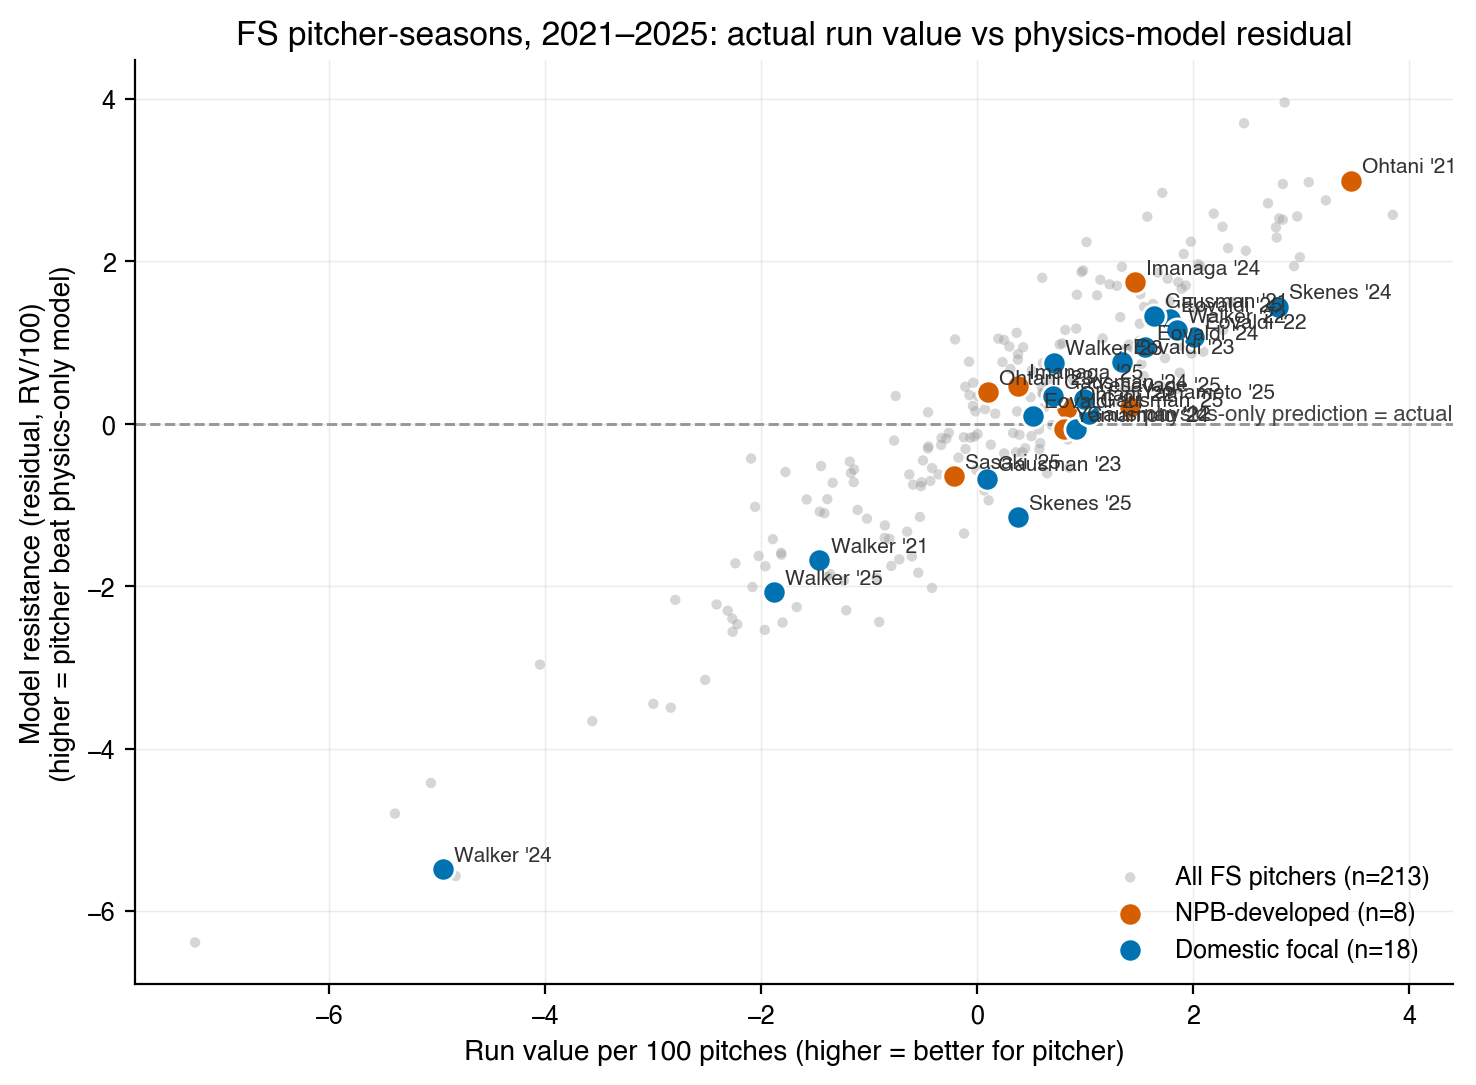
\includegraphics[width=0.86\linewidth]{fig01_residuals_landscape.png}
\caption{Splitter pitcher-seasons, 2021--2025 ($\geq$100 FS). Horizontal axis: run value per 100 pitches. Vertical axis: model resistance. Points above the dashed line beat the physics-only model. NPB-developed pitchers (vermillion) do not cluster above the domestic pitchers. Both axes derive from the same per-pitch target, so the diagonal trend is partly mechanical.}
\label{fig:landscape}
\end{figure}

\subsection{Splitter versus changeup}

Table~\ref{tab:coefs} reports both regressions.

\begin{table}[t]
\centering\small
\caption{Mixed-effects estimates of model resistance (RV/100). Standard errors are in parentheses. The \code{npb\_years} term is dropped for changeups because no NPB-developed pitcher reaches 100 changeups in any season.}
\label{tab:coefs}
\begin{tabular}{@{}lr@{\ }lr@{\ }l@{}}
\toprule
 & \multicolumn{2}{c}{Splitter (FS)} & \multicolumn{2}{c}{Changeup (CH)} \\
\midrule
\code{npb\_years}          & $0.101$  & $(0.100)$ & \multicolumn{2}{c}{---} \\
\code{mlb\_seasons\_in}    & $-0.053$ & $(0.033)$ & $0.002$  & $(0.015)$ \\
\code{fb\_velo}            & $0.053$  & $(0.051)$ & $0.029$  & $(0.020)$ \\
\code{usage\_share}        & $3.148^{**}$ & $(1.035)$ & $2.340^{***}$ & $(0.497)$ \\
\code{debut\_season}       & $-0.865^{*}$ & $(0.392)$ & $-0.127$ & $(0.173)$ \\
Intercept                  & $-5.371$ & $(4.905)$ & $-3.174$ & $(1.935)$ \\
\midrule
Pitcher variance $\hat\sigma_u^2$ & $0.347$ & $(0.163)$ & $0.142$ & $(0.064)$ \\
Residual variance $\hat\sigma^2$  & $2.196$ &  & $2.663$ & \\
Pitcher-seasons / pitchers & \multicolumn{2}{c}{239 / 111} & \multicolumn{2}{c}{1{,}166 / 520} \\
\bottomrule
\multicolumn{5}{@{}l}{\footnotesize $^{*}p<0.05$; $^{**}p<0.01$; $^{***}p<0.001$.}
\end{tabular}
\end{table}

\paragraph{Pitcher-specific variance.} The random-intercept variance is 0.347 for splitters and 0.142 for changeups, a ratio of about 2.4. After physics is accounted for, splitters show much more persistent pitcher-to-pitcher variation in model resistance than changeups do. Of the results here, this is the closest to Roberts' first claim: something pitcher-specific about the splitter escapes a physics-only model. It is a point estimate, and the variance components carry wide standard errors.

\paragraph{Debut-season penalty.} Pitchers in their MLB debut season underperform the model on splitters by 0.87 RV/100 (95\% CI $[-1.63, -0.10]$). On changeups the effect is a small, insignificant $-0.13$. The splitter appears to need adjustment time in the majors, whether by the pitcher, through learning to sequence it, or by the league, through scouting it. This runs against the popular story that NPB debutants outperform their peripherals. The debut-season population is mostly domestic rookies, and the five NPB pitchers are too few to move it.

\paragraph{Usage.} Pitchers who throw a pitch more often get more from it than physics predicts. Ten more percentage points of usage corresponds to about $+0.31$ RV/100 on splitters and $+0.23$ on changeups. The intervals overlap substantially (FS $[1.12, 5.18]$, CH $[1.37, 3.32]$), so the data supports a general off-speed specialization effect rather than a splitter-specific one. Causation could also run in reverse: pitchers throw their best pitches more.

\paragraph{The changeup comparison cannot test NPB development.} None of the five NPB-developed pitchers throws 100 changeups in any season, so \code{npb\_years} has no variation in the changeup sample. Whatever advantage these pitchers have, they express it through the splitter or forkball, not through off-speed pitching generally. The pitchers who develop the pitch specialize in it.

\subsection{Case studies}

Group-level inference is limited with five pitchers per group, but individual pitchers can be described in detail (Figures~\ref{fig:tunnels} and~\ref{fig:cases}).

\begin{figure}[t]
\centering
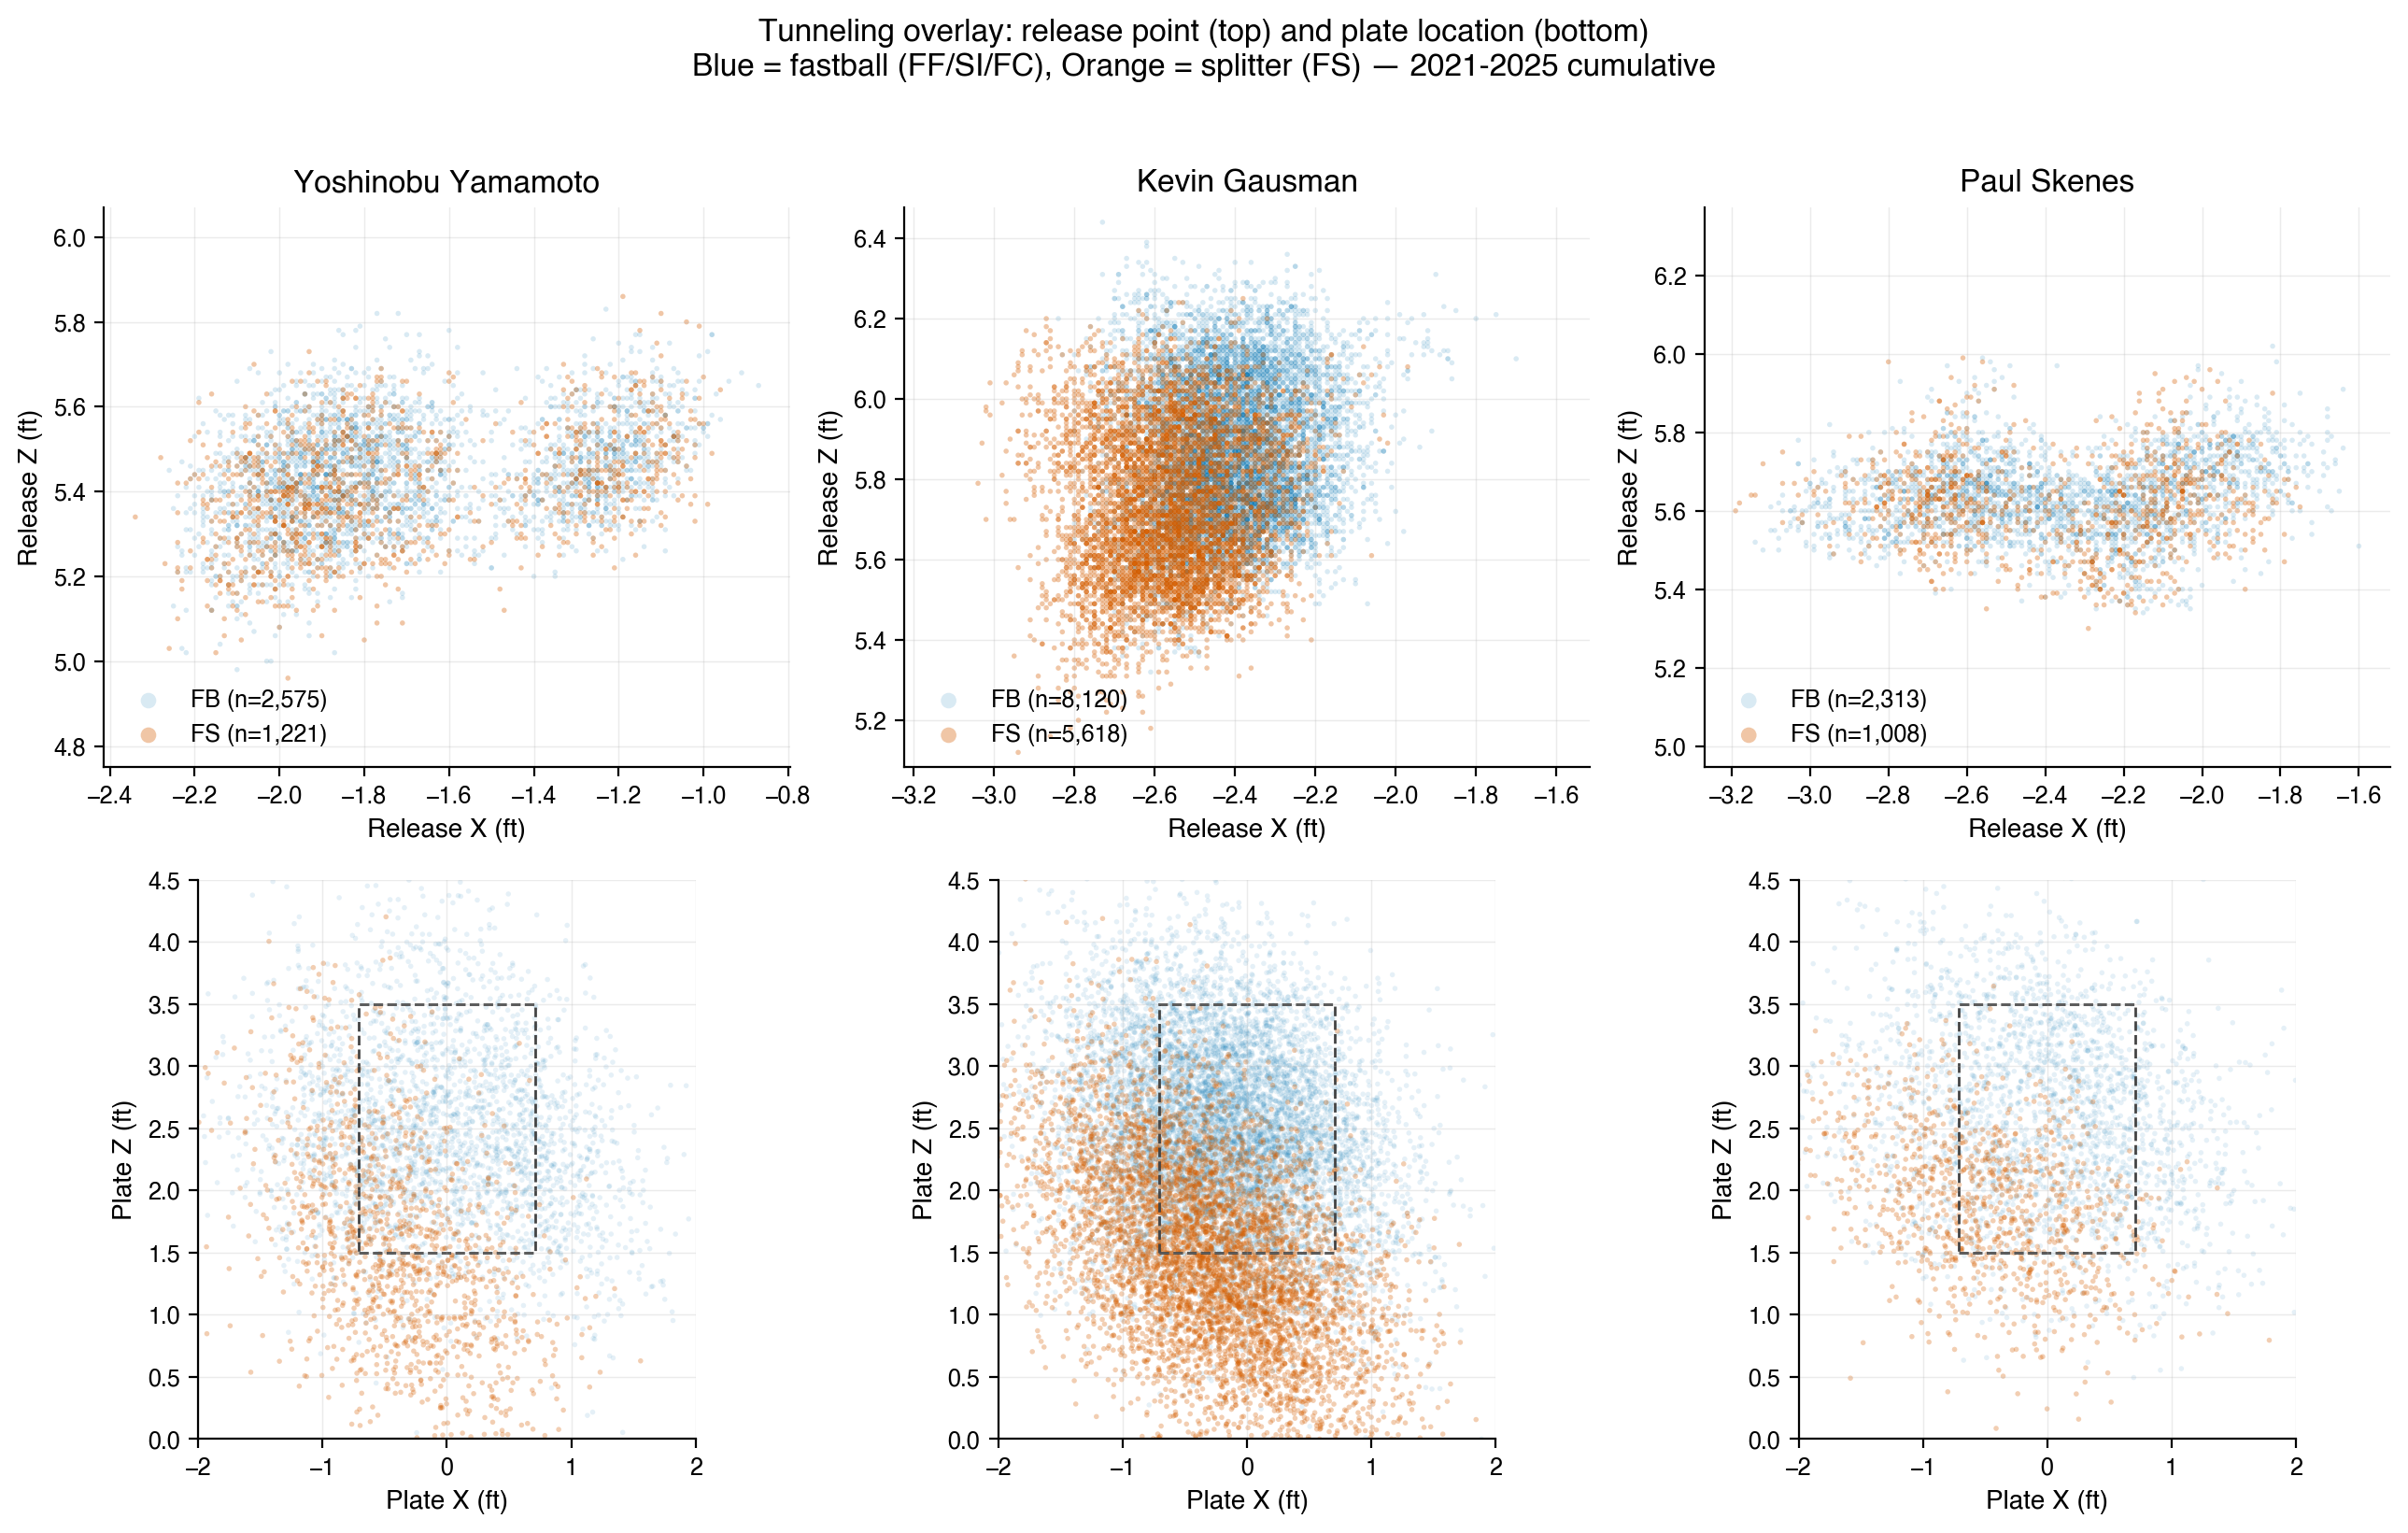
\includegraphics[width=\linewidth]{fig02_tunnels.png}
\caption{Release point (top) and plate location (bottom) for fastballs (blue) and splitters (orange), 2021--2025. Yamamoto's release points form two distinct clusters near $x \approx -2.0$ and $-1.4$ ft, consistent with an arm-slot change between 2024 and 2025.}
\label{fig:tunnels}
\end{figure}

\paragraph{Yoshinobu Yamamoto.} Model resistance is near zero in both seasons ($-0.06$ in 2024, $n=391$; $+0.21$ in 2025, $n=830$). His splitter is excellent, and the physics-only model already prices it correctly. The release-point clusters in Figure~\ref{fig:tunnels} suggest he used two distinct deliveries. Whether the two clusters differ in model resistance is untested.

\paragraph{Kevin Gausman.} His model resistance stays near zero across five seasons ($+1.33$, $-0.06$, $-0.67$, $+0.34$, $+0.12$). His splitter is elite in run value because of measurable physical traits. It shows no unmeasured edge and no resemblance to an NPB-style outlier.

\paragraph{Paul Skenes.} Model resistance fell from $+1.44$ in 2024 ($n=603$) to $-1.15$ in 2025 ($n=405$), the largest year-over-year change among focal pitchers. Possible explanations are hitter adaptation to a 94 mph splitter, a mechanical change, or first-year novelty that the model did not price. The present data cannot separate them. A two-component Gaussian mixture on velocity and fastball gap places Skenes in a ``splinker'' cluster (mean 87.5 mph, $-5.9$ mph gap) distinct from traditional splitters (85.7 mph, $-9.8$ mph). The v1 regression pools the two clusters.

\begin{figure}[t]
\centering
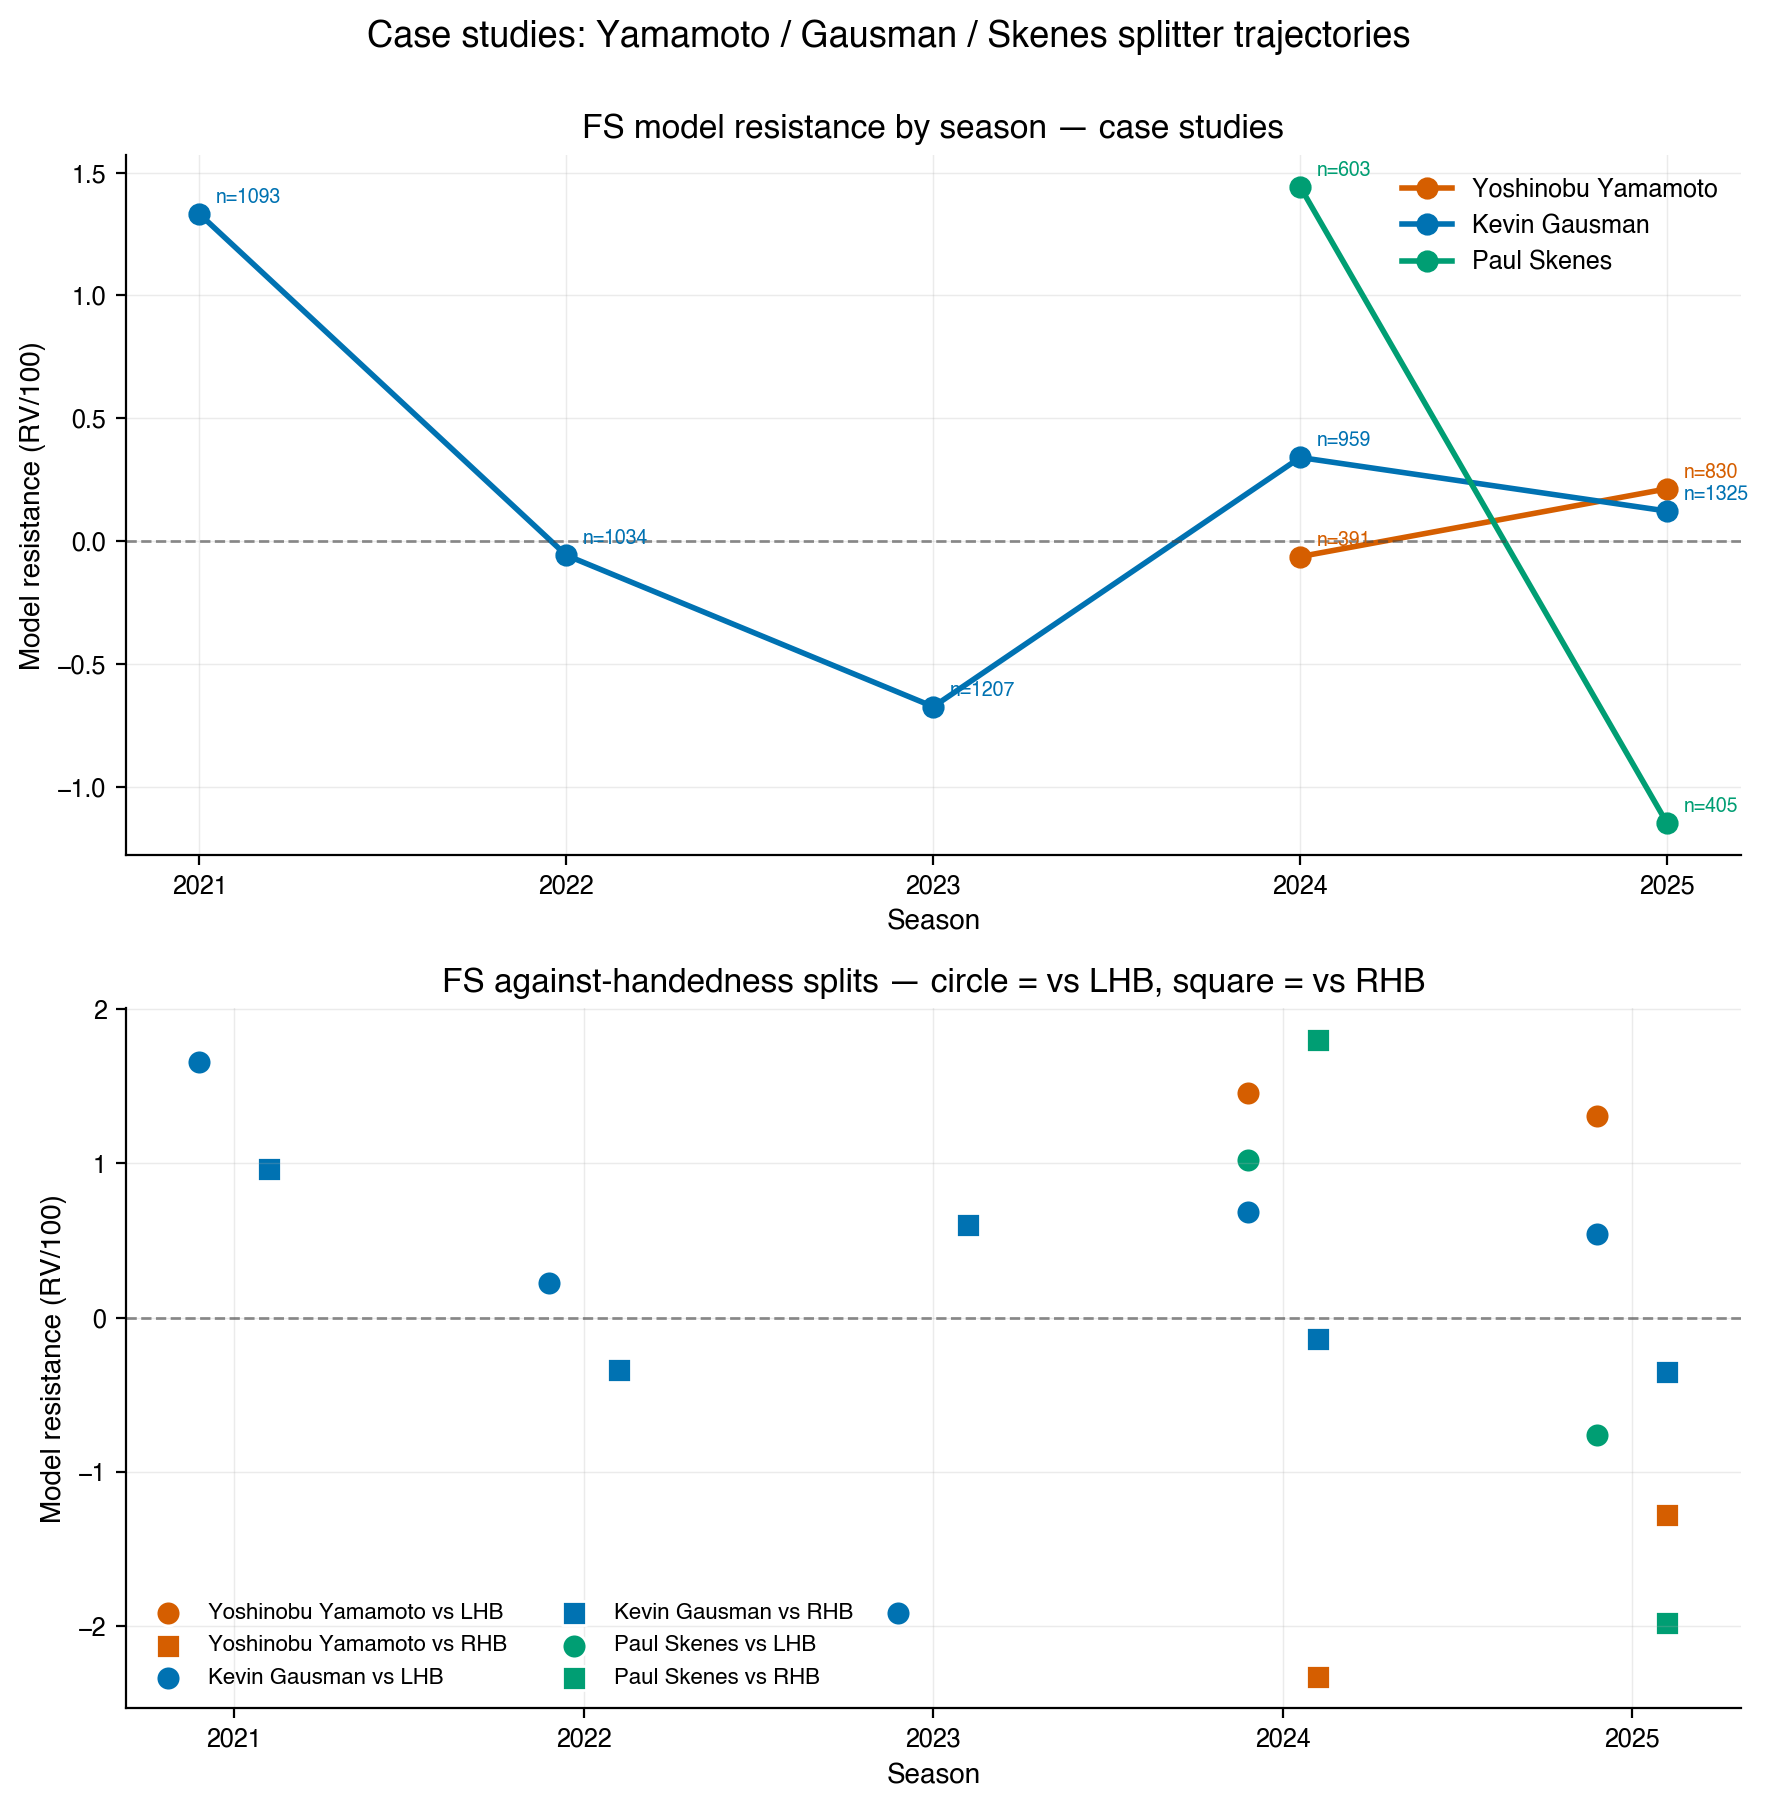
\includegraphics[width=0.78\linewidth]{fig03_case_studies.png}
\caption{Top: splitter model resistance by season for the three case-study pitchers. Bottom: splits against left-handed (circle) and right-handed (square) batters. Cell sizes in the bottom panel are small, so we draw no conclusions from it.}
\label{fig:cases}
\end{figure}

\paragraph{A sanity check.} Taijuan Walker's 2024 splitter has the most negative model resistance in the sample ($-5.49$ RV/100 over 318 pitches). Public run-value leaderboards ranked it the worst splitter in baseball that year. The residual decomposition reproduces that ranking without any information about it.

% ===========================================================================
\section{Limitations}

\begin{itemize}
\item \textbf{Association, not causation.} Only elite NPB pitchers reach MLB, and that selection cannot be modeled with available data.
\item \textbf{Hitter cognition is untested.} Claim (iii) requires bat-tracking or perceptual data.
\item \textbf{No NPB-side pitch data.} Translating NPB tracking data would introduce more error than it removes in a sample this small.
\item \textbf{Left-censoring.} For pitchers who debuted before 2021, career history before the window is unobserved.
\item \textbf{Pitch classification.} Statcast's \FS\ label pools traditional splitters with splinkers. Pooling may average over heterogeneous pitches.
\item \textbf{Variance-component uncertainty.} The 2.4$\times$ ratio has no interval yet.
\end{itemize}

% ===========================================================================
\section{What would change these conclusions}

\begin{itemize}
\item \textbf{NPB effect.} Adding the 2026 season yields a bootstrap interval on $\beta_1$ that excludes zero, or a Bayesian hierarchical refit with a weakly informative prior places more than 95\% posterior mass above zero.
\item \textbf{Splitter-specific variance.} A bootstrap of the variance components shows $\sigma_{u,\text{FS}}^2 > \sigma_{u,\text{CH}}^2$ in nearly all draws, and a third off-speed pitch (curveball or sweeper) resembles \CH\ rather than \FS.
\item \textbf{Debut penalty.} The penalty persists after stratifying traditional splitters and splinkers, and it does not appear on curveballs or sweepers.
\item \textbf{Skenes.} A within-season decomposition shows gradual decline (adaptation) rather than a step change (mechanics).
\item \textbf{Yamamoto.} His two release-point clusters show materially different model resistance, which would mean his apparent stability averages two different pitches.
\end{itemize}

% ===========================================================================
\section{Conclusion}

Roberts' claim holds in a specific form. A physics-only model leaves more pitcher-specific value unexplained for the splitter than for the changeup, and debut-season pitchers show a splitter penalty with no changeup counterpart. The data does not show that NPB development explains which splitters outperform the model. With five NPB-developed pitchers, the effect is too imprecisely estimated to confirm or exclude. The pitchers who learned the splitter in Japan throw it instead of a changeup. Measuring what they do differently will take more seasons of data and hitter-side measurements.

% ===========================================================================
\section*{Data and code availability}

All code, derived data and figures are at \url{https://github.com/KylanHuynh7/Split-Resurgence}. The pipeline design, data contracts and the full reproduction sequence are documented in \code{docs/design.md}. An earlier draft computed \code{usage\_share} against splitters plus changeups rather than all pitches, which overstated the difference between \FS\ and \CH. The estimates here use the corrected definition (design document, \S6.1).

\begin{thebibliography}{9}\small
\bibitem{passan2025} J.~Passan. Interview with Dave Roberts on the splitter. \emph{ESPN}, 2025.
\bibitem{pybaseball} J.~LeDoux and contributors. \code{pybaseball}: Pull current and historical baseball statistics using Python. \url{https://github.com/jldbc/pybaseball}.
\bibitem{chadwick} Chadwick Baseball Bureau. The Chadwick Bureau register. \url{https://github.com/chadwickbureau/register}.
\bibitem{xgboost} T.~Chen and C.~Guestrin. XGBoost: A scalable tree boosting system. In \emph{Proc.\ 22nd ACM SIGKDD Int.\ Conf.\ on Knowledge Discovery and Data Mining}, pp.\ 785--794, 2016.
\bibitem{statsmodels} S.~Seabold and J.~Perktold. Statsmodels: Econometric and statistical modeling with Python. In \emph{Proc.\ 9th Python in Science Conf.}, 2010.
\bibitem{cameron2008} A.~C. Cameron, J.~B. Gelbach and D.~L. Miller. Bootstrap-based improvements for inference with clustered errors. \emph{Review of Economics and Statistics}, 90(3):414--427, 2008.
\bibitem{field2007} C.~A. Field and A.~H. Welsh. Bootstrapping clustered data. \emph{Journal of the Royal Statistical Society: Series B}, 69(3):369--390, 2007.
\end{thebibliography}

\end{document}
